\documentclass{beamer}
\usetheme{Madrid}
%\usebeamercolor{Madrid-default}
\usepackage{array}
\usepackage{tikz}
\usetikzlibrary{shapes,arrows}
\usepackage[ruled,vlined]{algorithm2e}
\usetikzlibrary{fit}
\tikzset{
	comp/.style = {
		minimum width  = 8cm,
		minimum height = 4.5cm,
		text width     = 8cm,
		inner sep      = 0pt,
		text           = green,
		align          = center,
		font           = \Huge,
		transform shape,
		thick
	},
	monitor/.style = {draw = none, xscale = 18/16, yscale = 11/9},
	display/.style = {shading = axis, left color = black!60, right color = black},
	ut/.style      = {fill = gray}
}
\tikzset{
	computer/.pic = {
		% screen (with border)
		\node(-m) [comp, pic actions, monitor]
		{\phantom{\parbox{\linewidth}{\tikzpictext}}};
		% display (without border)
		\node[comp, pic actions, display] {\tikzpictext};
		\begin{scope}[x = (-m.east), y = (-m.north)]
			% filling the lower part
			\path[pic actions, draw = none]
			([yshift=2\pgflinewidth]-0.1,-1) -- (-0.1,-1.3) -- (-1,-1.3) --
			(-1,-2.4) -- (1,-2.4) -- (1,-1.3) -- (0.1,-1.3) --
			([yshift=2\pgflinewidth]0.1,-1);
			% filling the border of the lower part
			\path[ut]
			(-1,-2.4) rectangle (1,-1.3)
			(-0.9,-1.4) -- (-0.7,-2.3) -- (0.7,-2.3) -- (0.9,-1.4) -- cycle;
			% drawing the frame of the whole computer
			\path[pic actions, fill = none]
			(-1,1) -- (-1,-1) -- (-0.1,-1) -- (-0.1,-1.3) -- (-1,-1.3) --
			(-1,-2.4) coordinate(sw)coordinate[pos=0.5] (-b west) --
			(1,-2.4) -- (1,-1.3) coordinate[pos=0.5] (-b east) --
			(0.1,-1.3) -- (0.1,-1) -- (1,-1) -- (1,1) -- cycle;
			% node around the whole computer
			\node(-c) [fit = (sw)(-m.north east), inner sep = 0pt] {};
		\end{scope}
	}
}
\makeatother
\setbeamertemplate{footline}
{
	\leavevmode%
	\hbox{%
		\begin{beamercolorbox}[wd=.4\paperwidth,ht=2.25ex,dp=1ex,center]{author in head/foot}%
			\usebeamerfont{author in head/foot}\insertshortauthor
		\end{beamercolorbox}%
		\begin{beamercolorbox}[wd=.6\paperwidth,ht=2.25ex,dp=1ex,center]{title in head/foot}%
			\usebeamerfont{title in head/foot}\insertshorttitle\hspace*{3em}
			\insertframenumber{} / \inserttotalframenumber\hspace*{1ex}
	\end{beamercolorbox}}%
	\vskip0pt%
}
\makeatletter
\setbeamertemplate{navigation symbols}{}


\title[Federated Learning]{Federated Learning}

\author{Hoang Trung Hieu}
\centering
\date{2020}

\begin{document}
\maketitle
\begin{frame}{What is the fererated learning?}
	



\begin{center}
	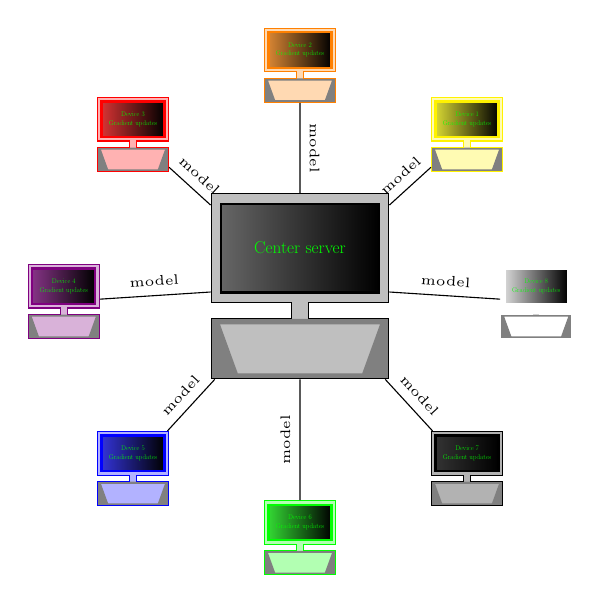
\begin{tikzpicture}
		\pic(comp0) [
		draw,
		fill = gray!50,
		scale = 0.25,
		pic text = {Center server}
		]
		{computer};
		\path(comp0-c.center) pic 
		foreach[count=\i] \farbe in {yellow, orange, red, red!50!blue, blue, green, black,white}
		(comp\i) [
		draw = \farbe,
		fill = \farbe!30,
		display/.append style = {left color=\farbe!80!black!80},
		scale = 0.1,
		pic text = {Device \i \\Gradient updates}		
		] at +(45*\i:3){computer};	
		\foreach \i in {1,2,3,4,5,6,7,8} \draw (comp\i-c) -- (comp0-c)  node [midway, above, sloped] (TextNode) {\tiny{model}};
		
	\end{tikzpicture}
\end{center}
\end{frame}
\begin{frame}{Challenges in fererated learning} 
 \begin{itemize}
 \item \textit{Massively distributed}. The number of mobile device owners is massively bigger than average of the number of training samples on each device.
 \item \textit{Unbalanced}. Some users produce significantly more data than others.
 \item \textit{Non-IID}.	The data generated by each user are quite different.
 \end{itemize}
\end{frame}
\begin{frame}{Problem description} 
		\begin{flushleft}
			Let us consider the following distributed optimization model in which $N$ clients cooperatively solve  $$\min_{w} f(w) = \min_{w} \sum_{k=1}^{N} p_k f_k(w)$$
	where $p_k$ be the weight of $k-$th device , $p_k \ge 0, \quad  \sum_{i=1}^{N}p_k=1.$\\ The $k-$th client has $n_k$ training data which is denoted $x_{k,1} , \cdots,  x_{k,n_k}.$ The local generalization error function are defined by $$f_k(w)= \frac{1}{n_k} \sum_{j=1}^{n_k} \ell (w;x_{k,j})$$
	where $\ell$ is a user loss function of the prediction.	
		\end{flushleft}
\end{frame}

\begin{frame}{Federated Averaging Algorithms}
			\begin{algorithm}[H]
			\SetAlgoLined
			\textbf{Server executes:} 	Initialization $w_0$ \;
			\For{each round $t=1,2, \cdots $}{
				$m \leftarrow \max(C \cdot K,1)$\\
				$S_t \leftarrow $ (random set of $m$ client) \\
				\For{each client $k \in S_t$} {	
					$w_{t+1}^k \leftarrow \text{ClientUpdate}(k, w_t)$\;			
				}{
					$w_{t+1} \leftarrow \sum_{k=1}^{K} \dfrac{n_k}{n} w_{t+1}^k$\;
				}
			} 
			\textbf{ClientUpdate($k,w$):}\\
			$B \leftarrow \text{ (split} \ P_k	\ \text{into batches of size} \ B )$\\
			\For{each local epoch}{
				\For{batch $b \in B$}{
					$ w \leftarrow w - \eta \nabla \l(w;b)$ }}
			\caption{FederatedAveraging(FedAvg).}
		\end{algorithm}
		
\end{frame}
\begin{frame}{Experiments-Input
	}
	Real data: MNIST\\
\begin{center}
	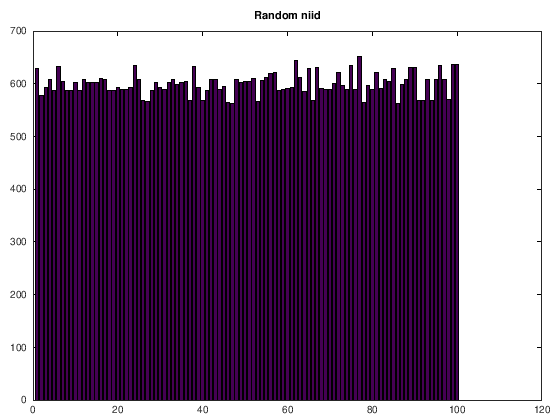
\includegraphics[scale=0.3]{random_niid.png}
	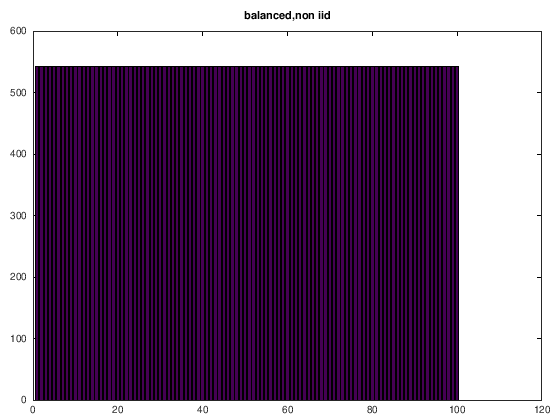
\includegraphics[scale=0.3]{equal.png}\\
	\figurename{. Unbalanced (left) and balanced (right) data distribution}
\end{center}
	\end{frame}

\begin{frame}{Experiments-Input}
	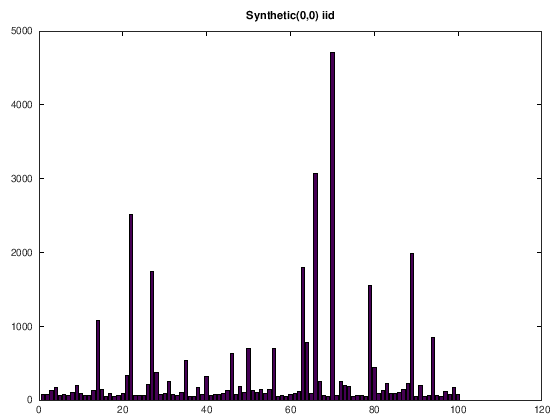
\includegraphics[scale=0.2]{sy00iid.png}
	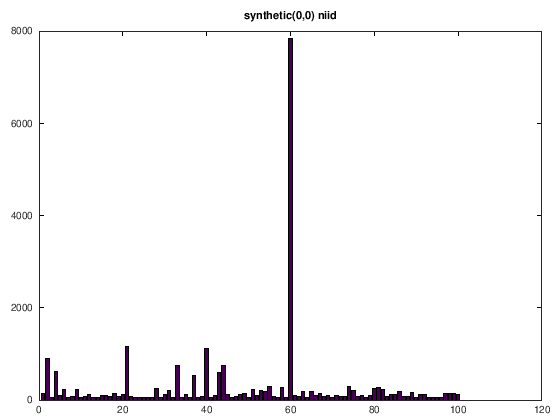
\includegraphics[scale=0.2]{sy00niid.png}
	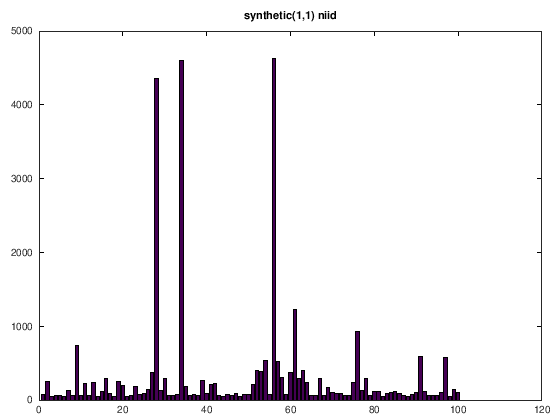
\includegraphics[scale=0.2]{sy11.png}
	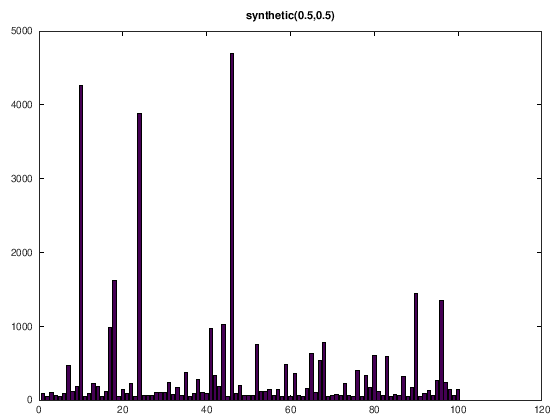
\includegraphics[scale=0.2]{sy0.50.5.png}\\
	\figurename[1.2]{. Synthetic data with $(\alpha, \beta) =(0,0)$-iid ,$(\alpha, \beta) =(0,0)$-niid,$(\alpha, \beta) =(1,1)$-niid,$(\alpha, \beta) =(0.5,0.5)$-niid }\\
\end{frame}

\begin{frame}{Experiments-Models}
	\begin{block}{2NN}
	(fc1): Linear( input features=784, output features=200, bias=True)\\
	(fc2): Linear( input features=200, output features=200, bias=True)\\
	(fc3): Linear(input features=200, output features=10, bias=True)
	\end{block}
\begin{block}{CNN}
	(conv1): Conv2d(1, 32, kernel size=(5, 5), stride=(1, 1)) \\
	(conv2): Conv2d(32, 64, kernel size=(5, 5), stride=(1, 1))\\
	(fc 1): Linear(input features=1024, output features=512, bias=True)\\
	(fc 2): Linear(input features=512, output features=10, bias=True)
	\end{block}
\end{frame}
\begin{frame}{Experiments-Results}
 Synthetic(0,0) iid (right) and non-iid (left) dataset, $ B=64, T=50,lr=0.01,E=5$, model is 2NN. The value of $C$ in the set $\{5/100,10/100,20/100,50/100\}$. The horizontal axis is the train loss.
\begin{center}
	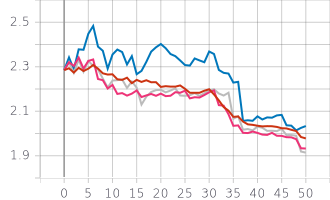
\includegraphics[scale=0.5]{Cniid.png}
	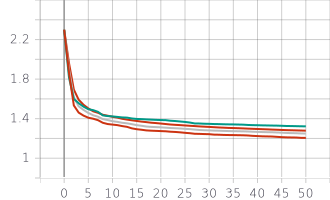
\includegraphics[scale=0.5]{Ciid.png} \\
	\figurename[3.1]{. Impact of C}
\end{center}
\end{frame}
\begin{frame}{Experiments-Results}
 MNIST unbalanced non-iid dataset, $C=5/100, B=64, T=50,lr=0.01$, model is CNN. The value of $E$ in the set $\{2,5,10,20\}$. The horizontal axis is the train accuracy.
\begin{center}
	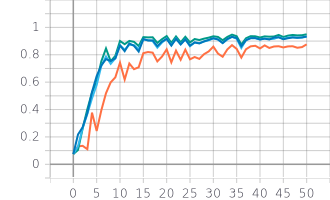
\includegraphics[scale=0.65]{E.png}\\
	\figurename[3.2]{. Impact of E}
\end{center}
\end{frame}
\begin{frame}{Experiments-Results}
To evaluate the impact of batch size, we examine on MNIST balanced non-iid dataset, $C=10/100, T=50,lr=0.01$, model is 2NN. The value of $B$ in the set $\{16,32,64,128\}$. The horizontal axis is the test accuracy.
\begin{center}
	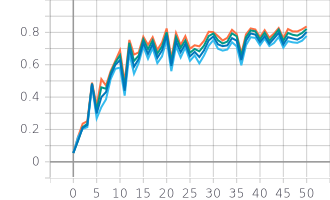
\includegraphics[scale=0.65]{B.png}\\
	\figurename[3.3]{. Impact of B}
\end{center}
\end{frame}
\begin{frame}{Experiments-Results}
\textbf{Impact of balancedness.}
	  Synthetic data with $(\alpha, \beta) =(0,0)$-iid ,$(\alpha, \beta) =(0,0)$-niid,$(\alpha, \beta) =(1,1)$-niid,$(\alpha, \beta) =(0.5,0.5)$-niid $C=10/100, B=64, T=50,lr=0.01, E=5$, model is CNN. The horizontal axis is the test loss.
\begin{center}
	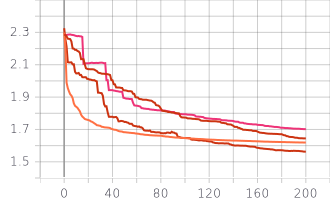
\includegraphics[scale=0.65]{syn.png}\\
	\figurename[3.4]{. Impact of unbalancedness}
\end{center}
\end{frame}

\begin{frame}

THANK YOU FOR YOUR ATTENTION!
\end{frame}



\end{document}
